\documentclass[12pt]{article}

\usepackage{fullpage, amsmath, amssymb, amsthm, setspace, graphicx, grffile}
\usepackage{xfrac}
\usepackage{subcaption}
\usepackage{float}
\usepackage{tikz, tikz-cd}
\usetikzlibrary{graphs,graphs.standard, arrows}
\usetikzlibrary{decorations.markings,plotmarks}
\usepackage{ upgreek }
\newtheorem{theorem}{Theorem}[section]
\newtheorem{lemma}[theorem]{Lemma}
\newtheorem{conjecture}[theorem]{Conjecture}
\newtheorem{condition}[theorem]{Condition}
\newtheorem{claim}[theorem]{Claim}
\newtheorem{question}[theorem]{Question}
\newtheorem{corollary}[theorem]{Corollary} 
\newtheorem{proposition}[theorem]{Proposition}
\theoremstyle{definition}
\newtheorem{definition}[theorem]{Definition}
\newtheorem{statement}[theorem]{Statement}
\newtheorem{notation}[theorem]{Notation} 
\newtheorem{construction}[theorem]{The Construction}
\newtheorem{remark}[theorem]{Remark}
\newtheorem{example}[theorem]{Example} 

 \usepackage{amsmath}
    \usepackage{amssymb}
    \usepackage{amsthm}
    \usepackage{amsfonts}
    \usepackage{braket}
\definecolor{dkgreen}{rgb}{0,0.6,0}
\definecolor{gray}{rgb}{0.5,0.5,0.5}
\definecolor{mauve}{rgb}{0.58,0,0.82}
\usepackage{listings}
\lstset{frame=tb,
  language=Java,
  aboveskip=3mm,
  belowskip=3mm,
  showstringspaces=false,
  columns=flexible,
  basicstyle={\small\ttfamily},
  numbers=none,
  breaklines=true,
  breakatwhitespace=true,
  tabsize=3
}
\begin{document}


\title{Deutsch-Jozsa Algorithm}

\author{Aaron Baxter}
\date{April 19, 2020}

\maketitle
\section{About the Creators}
The Deutsch-Jozsa algorithm was created by quantum physicist David Deutsch and mathematicion Richard Jozsa. Deutsch is considered to be the one the founding fathers of quantum computing. Born in Haifa, Israel, he attended the University of Cambridge and the University of Oxford. He currently teaches at the University of Oxford and is the founding member of the Centre for Quantum Computation at Clarendon Laboratory at Oxford. He currently does not accept a paid position at Oxford, where he is considered a ``non-stipendiary Visiting Professor of Physics at the University of Oxford". He has various accolades, notably, the Micius Quantum Prize in 2018 as well as being elected a Fellow of the Royal Society in 2008.
 \vspace{.2 in}
 
 
 \noindent Richard Jozsa is a mathematician from Australia. Josza studied at the University of Oxford. He is currently a physics professor at the University of Cambridge. Josza is credited as one of the founders of quantum teleportation. He is the holder of the Leigh Trapnell Chair in Quantum Computing. Like Deutsch, he was elected a Fellow of the Royal Society in 2019. 
 
 \section{Introduction}
 \noindent The Deutsch-Jozsa algorithm was created in order to show that a quantum computer can solve the same algorithm faster than classical computer can. The Deutsch-Jozsa algorithm is considered by many to be the ``Hello World!" of quantum algorithms. The function for the algorithm is as follows:
 \begin{definition}
 The function for the algorithm s.t. $n\in\mathbb{Z^+}$:
 \[f: \{0,1\}^n\longrightarrow\{0,1\}\]
 We are promised that the function is either \textbf{constant} or \textbf{balanced}.
 \end{definition}
 \vspace{.2 in}
 \begin{definition}
 F is a \textbf{constant function} if and only if $f(x) = 0$ for every $x\in\{0,1\}^n$ or $f(x) = 1$ for every $x\in\{0,1\}^n$. For example:
 
\begin{table}[H]
    \begin{minipage}{.5\linewidth}
      \centering
        \begin{tabular}{|c|c|}
           \hline
            x&f(x)\\
            \hline
            00 & 0  \\  
            01 & 0 \\
            10 & 0 \\
            11 & 0 \\
            \hline
        \end{tabular}
        \caption{output 0}
    \end{minipage}%
    \begin{minipage}{.5\linewidth}
      \centering
        
        \begin{tabular}{|c|c|}
         \hline
            x&f(x)\\
            \hline
            00 & 1  \\  
            01 & 1 \\
            10 & 1 \\
            11 & 1 \\
            \hline
        \end{tabular}
        \caption{output 1}
    \end{minipage} 
\end{table}

\end{definition}
 \begin{definition}
 F is a \textbf{balanced function} if and only if $f(x) = 0$ for half of all $x\in\{0,1\}^n$ and $f(x) = 1$ for half of all $x\in\{0,1\}^n$. For example:
\begin{table}[H]
    \begin{minipage}{.5\linewidth}
      
      \centering
        \begin{tabular}{|c|c|}
           \hline
            x&f(x)\\
            \hline
            00 & 0  \\  
            01 & 0 \\
            10 & 1 \\
            11 & 1 \\
            \hline
        \end{tabular}
        \caption{output 0,1}
    \end{minipage}%
    \begin{minipage}{.5\linewidth}
      \centering
        
        \begin{tabular}{|c|c|}
         \hline
            x&f(x)\\
            \hline
            00 & 0  \\  
            01 & 1 \\
            10 & 0 \\
            11 & 1 \\
            \hline
        \end{tabular}
        \caption{output 0,1}
    \end{minipage} 
\end{table}
\end{definition}
\section{Classical Runtime of the Algorithm}
In order to find whether the algorithm is balanced or constant in classical time, we would need to check $f(x)$ for every bit. Let n be the number of qubits represented in the algorithm. Thus $2^n= \text{number of bits}$. 
\begin{theorem}
The worst case number of steps for classically computing the Deutsch-Jozsa algorithm takes $2^{n-1}+1$ steps.
\end{theorem}
\begin{example}
Let $n=2$. Let the Deutsch-Jozsa algorithm contain a function where the function output ($f(x)$) of $\ket{00}$ and $\ket{01}$ is 0. 
 
\begin{center}
\begin{tabular}{|c|c|} 
 \hline
 x & f(x) \\ 
 \hline
 00 & 0 \\ 
 01 & 0 \\ 
 \vdots & \vdots\\
 \hline
\end{tabular}
\end{center}
Remember, the Deutsch-Jozsa algorithm \emph{promises} us that the function is either constant or balanced. At this point, we cannot determine if the function is constant or balanced. If $x = \ket{10}$ and $f(x)=0$, then we must conclude that the function is constant. If $f(x)=1$, then we can determine the function is balanced. This would mean one more than half of all the bits were compared. We can make a conclusion once we have compared one more than half. By Theorem 3.1, since $n=2$ then $2^{1}+1=3$. Thus at the worst case when $n=2$, it will take three bits to tell us if the function is constant or balanced. The range of steps to compute the algorithm when $n=2$ is $2\leq x\leq 2^{n-1}+1$
\end{example}
\section{Circuit Construction of Algorithm}
\begin{center}
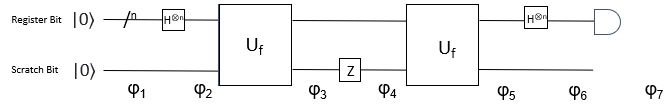
\includegraphics[]{circuit.PNG}
\end{center}
The \textit{Register} bits are passed through a Hadamard gate which puts them into a superposition state. Both the \textit{Scratch} and \textit{Register} bits are passed through the oracle function. The \textit{Scratch} bit's work is passed through a Z gate and then passed through the oracle function again in order erase the work done to it. The \textit{Register} bits are then passed through a Hadamard gate and their bits are read. The scratch bit is essentially ``thrown out". The lowercase phis represent the stages of the circuit. \emph{Eisuke Abe's} presentation on the Deutsch-Jozsa Algorithm \footnote{https://www.appi.keio.ac.jp/Itoh_group/abe/pdf/qc3.pdf} demonstrates the equations below needed to interpret the circuit:
\begin{itemize}
\item $H^{\otimes n}\ket{x} = \dfrac{1}{2^{n/2}}\sum_{x = 0}\ket{x}= \dfrac{1}{2^{n/2}}\sum_{z}(-1)^{x\cdot z}\ket{z}$
\item $U_f\ket{x}\ket{y}=\ket{x}\ket{y\oplus f(x)}$
\item $Z\ket{y} = (-1)^y\ket{y}$
\end{itemize}
thus:
\begin{itemize}
\item $\upvarphi_1 = \ket{0}\ket{0}$ 
\item $\upvarphi_2 = \dfrac{1}{2^{n/2}}\sum_{x}\ket{x}\ket{0}$ 
\item $\upvarphi_3 = \dfrac{1}{2^{n/2}}\sum_{x}\ket{x}\ket{f(x)}$ 
\item $\upvarphi_4 = \dfrac{1}{2^{n/2}}\sum_{x}(-1)^{f(x)}\ket{x}\ket{f(x)}$
\item $\upvarphi_5 = \dfrac{1}{2^{n/2}}\sum_{x}(-1)^{f(x)}\ket{x}\ket{0} $
\item $\upvarphi_6 = \sum_z\sum_x\dfrac{(-1)^{f(x)+x\cdot z}}{2^n}\ket{z}\ket{0}$
\end{itemize}
We use this equation to classify the function 
$\sum_x\dfrac{(-1)^{f(x)}}{2^n}\ket{z}$
\begin{itemize}
\item $\upvarphi_7$ = 
   $ \sum_x\dfrac{(-1)^{f(x)}}{2^n}= 
    \begin{cases}
      0, & \text{balanced} \\
      \pm1, & \text{constant}
    \end{cases}$
\end{itemize}
\begin{example}
If the function is \textbf{constant}, then $f(x) =0$ and the solution is equal to $1$. We will show this below where $n=3$.
\[\sum_{x=0}^{7}\dfrac{(-1)^{f(x)}}{2^3}= \dfrac{(-1)^0+(-1)^0+(-1)^0+(-1)^0+(-1)^0+(-1)^0+(-1)^0+(-1)^0}{8}=1\]
\end{example}
\begin{example}
If the function is balanced, then $f(x) =0$ half of the time, and $f(x) = 1$ the other half. The solution is equal to 0. Because half of the $-1s$ have a $0$ as an exponent, those will equal $1$. When they exponent is a $1$, they will equal $-1$. Because there are half of each, they offset to equal $0$.We will show this below where $n=3$.
\[\sum_{x=0}^{7}\dfrac{(-1)^{f(x)}}{2^3}= \dfrac{(-1)^0+(-1)^1+(-1)^0+(-1)^1+(-1)^0+(-1)^0+(-1)^1+(-1)^1}{4}=0\]
\end{example}


\section{Simplified Deutsch-Jozsa circuit}
If the algorithm only takes in 2 qubits, the circuit of the Deutsch-Josza algorithm can be simplified. The scratch bit is initialized at $1$ instead of starting at $0$. The READ gate will read the output of $(f(0) \oplus f(1))$. If the READ gate reads a $0$ and $f(x)$ equals $0$ for all 0s or $1$ for all 1s, then the function is \textbf{constant}. If the READ gate reads a $1$ and $f(x)$ equals $1$ half of the outputs and $0$ the other half, then the function is \textbf{balanced}.

\begin{center}
    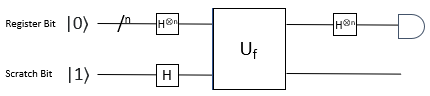
\includegraphics[]{revised.PNG}
\end{center}


\noindent Let's represent the oracle with logic gates and their matrix equivalent. I will be using the QCEngine to show circuits which demonstrate how the matrix and logic gates are implemented. Constant functions can be represented using two different oracles. Balanced functions can also be represented using two different oracles. Note that in the outputs of the multi-qubit registers, the phase carries no bearing on whether the function is constant or balanced. 
\begin{example}
In this \textbf{constant} circuit, we use the NOT gate on $0x2$.
\begin{center}
    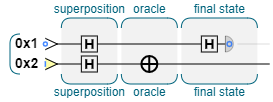
\includegraphics[]{cona1.PNG}
\end{center}



\noindent The NOT gate on $0x2$ can be represented in a 2-qubit system in a matrix as $\begin{bmatrix}
0&0&1&0\\
0&0&0&1\\
1&0&0&0\\
0&1&0&0\\
\end{bmatrix}$. We will do an example with this matrix later on.
The output on a multi-qubit system contains only 0s in the $2^0$ column. Since the READ gate only reads from the $2^0$ column($0x1$), the circuit will read $0$ $100\%$ of the time, thus \textbf{constant}. Output:

\vspace{.2 cm}
\begin{center}
    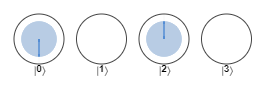
\includegraphics[]{cona2.PNG}
\end{center}
\end{example}
\vspace{.5 cm}

\begin{example}
In this \textbf{constant} circuit, the oracle function does not contain a logic gate.

\begin{center}
    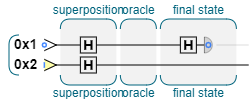
\includegraphics[]{conb1.PNG}
\end{center}
\vspace{.4 cm}
\noindent Because we don't use a logic gate, we can represent this through an Identity matrix \begin{bmatrix}
1&0&0&0\\
0&1&0&0\\
0&0&1&0\\
0&0&0&1\\
\end{bmatrix}
The output on a multi-qubit system contains only 0s in the $2^0$ column. The READ gate only reads from the $2^0$ column ($0x2$), therefore, the circuit will read $0$ $100\%$ of the time, thus \textbf{constant}. Output:

\vspace{.2 cm}
\begin{center}
   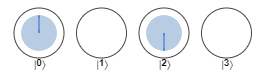
\includegraphics[]{conb2.PNG} 
\end{center}
\end{example}
\vspace{.5 cm}

\begin{example}
In this \textbf{balanced} circuit, we use a CNOT gate with target on $0x2$.

\begin{center}
   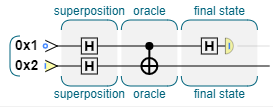
\includegraphics[]{bala1.PNG} 
\end{center}


\vspace{.4 cm}
\noindent The CNOT gate with target on $0x2$ can be represented in a 2-qubit system in matrix \begin{bmatrix}
1&0&0&0\\
0&0&0&1\\
0&0&1&0\\
0&1&0&0\\
\end{bmatrix}.
The output on a multi-qubit system contains only 1s in the $2^0$ column. The READ gate only reads from the $2^0$ column ($0x1$), therefore, the circuit will read $1$ $100\%$ of the time, thus \textbf{balanced}. Output:

\vspace{.2 cm}
\begin{center}
    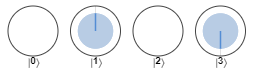
\includegraphics[]{bala2.PNG}
\end{center}

\end{example}
\vspace{.5 cm}

\begin{example}
In this balanced circuit, we use a NOT gate on $0x2$ and CNOT gate with target on $0x2$ and control on $0x1$.

\begin{center}
    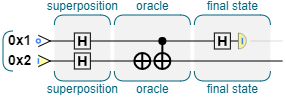
\includegraphics[]{balb2.PNG}
\end{center}

\vspace{.4 cm}
\noindent The oracle's gates can be represented in a 2-qubit system in matrix \begin{bmatrix}
0&0&1&0\\
0&1&0&0\\
1&0&0&0\\
0&0&0&1\\
\end{bmatrix}.
The output on a multi-qubit system contains only 1s in the $2^0$ column. The READ gate only reads from the $2^0$ column, therefore, the circuit will read $1$ $100\%$ of the time, thus \textbf{balanced}. Output:

\vspace{.2 cm}
\begin{center}
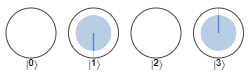
\includegraphics[]{balb1.PNG}
\end{center}
\end{example}
\vspace{.5 cm}

\section{Example}
Lets do an example with two qubits. Let there be a constant function st the oracle function is represented by a NOT gate on $0x2$. We can represent the circuit by:

\begin{center}
    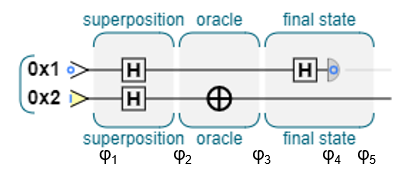
\includegraphics[]{example.PNG}
\end{center}

We will do the matrix multiplication and solve this in phases as we did when we interpreted the circuit. 

\begin{itemize}

\item $\upvarphi_1:$ $\ket{10}$ can be represented with the column vector $\begin{bmatrix}
0\\
0\\
1\\
0\\
\end{bmatrix}$ 
\item $\upvarphi_2:$ when we put the qubits in a superposition state, we have to mutiply the column vector by the Hadamard matrix:
\[\begin{bmatrix}
\sfrac{1}{2}& \quad\sfrac{1}{2}&\quad\sfrac{1}{2}& \quad\sfrac{1}{2}\\
\sfrac{1}{2}&\sfrac{-1}{2}&\quad \sfrac{1}{2}&\sfrac{-1}{2}\\
\sfrac{1}{2}&\quad\sfrac{1}{2}&\sfrac{-1}{2}&\sfrac{-1}{2}\\
\sfrac{1}{2}&\sfrac{-1}{2}&\sfrac{-1}{2}&\quad\sfrac{1}{2}\\
\end{bmatrix}
\cdot
\begin{bmatrix}
0\\
0\\
1\\
0\\
\end{bmatrix}
=
\begin{bmatrix}
\quad\sfrac{1}{2}\\
\quad\sfrac{1}{2}\\
\sfrac{-1}{2}\\
\sfrac{-1}{2}\\
\end{bmatrix}\]
\item $\upvarphi_3:$ Applying the NOT gate's matrix (on $0x2$ to the new column vector, we get: 
\[
\begin{bmatrix}
0&0&1&0\\
0&0&0&1\\
1&0&0&0\\
0&1&0&0\\
\end{bmatrix}
\cdot
\begin{bmatrix}
\quad\sfrac{1}{2}\\
\quad\sfrac{1}{2}\\
\sfrac{-1}{2}\\
\sfrac{-1}{2}\\
\end{bmatrix}
=
\begin{bmatrix}
\sfrac{-1}{2}\\
\sfrac{-1}{2}\\
\quad\sfrac{1}{2}\\
\quad\sfrac{1}{2}\\
\end{bmatrix}
\]

\item $\upvarphi_4:$ We then apply the Hadamard gate to only $0x1$. We form the Hadamard's matrix by $I_2 \otimes H$ where $H$ is the 2x2 Hadamard matrix. We multiply the resulting matrix to the column vector:
\[
\begin{bmatrix}
\sfrac{1}{\sqrt{2}}&\quad\sfrac{1}{\sqrt{2}}&0&\quad0\\
\sfrac{1}{\sqrt{2}}&\sfrac{-1}{\sqrt{2}}&0&\quad0\\
0&\quad0&\sfrac{1}{\sqrt{2}}&\quad\sfrac{1}{\sqrt{2}}\\
0&\quad0&\sfrac{1}{\sqrt{2}}&\sfrac{-1}{\sqrt{2}}\\
\end{bmatrix}
\cdot
\begin{bmatrix}
\sfrac{-1}{2}\\
\sfrac{-1}{2}\\
\quad\sfrac{1}{2}\\
\quad\sfrac{1}{2}\\
\end{bmatrix}
=
\begin{bmatrix}
\sfrac{-1}{\sqrt{2}}\\
\quad0\\
\quad\sfrac{1}{\sqrt{2}}\\
\quad0\\
\end{bmatrix}
\]
\item $\upvarphi_5:$ Now we read the $0x1$ bit. Let's set up the table of possible bits for 2 qubits and bold the bits represented in our example. 

\begin{center}
\begin{tabular}{|c|c|} 
 \hline
 0x2&0x1 \\ 
 \hline
 \textbf{-0}&\textbf{0} \\ 
 0&1\\ 
 \textbf{1}&\textbf{0}\\
 1&1\\
 \hline
\end{tabular}
\end{center}

Since the read function represents what the output of $f(0) \oplus f(1)$ and the output equals 0, the function in our example is \textbf{constant}.
\end{itemize}


\clearpage
\section{QCEngine code used to create circuits}

\begin{lstlisting}
    qc.clearOutput()
    qc.reset(2)
    qc.had()
    var x = qc.read() //creating number 0-3 to determine oracle function
    qc.reset(2)
    qc.write(2)
    superposition()
    var y = oracle(x) 
    state(y)
    
    function superposition() {
        qc.label('superposition')
        qc.nop()
        qc.had()
        qc.nop()
        qc.label()
    }
    
    function oracle(x){
        qc.label('oracle')
        qc.nop()
        switch(x) {
            case 0:
                break
            case 1:
                qc.not(0x2)
                break
            case 2:
                qc.cnot(0x2,0x1)
                break
            case 3:
                qc.not(0x2)
                qc.cnot(0x2,0x1)
                break
        }
        qc.nop()
        qc.label()
        return x
        
    }
    
    function state(y){
        qc.label('final state')
        qc.nop()
            switch(y) {
            case 0:
                qc.had(0x1)
                qc.print('Constant\n')
                qc.print('Output: ' + qc.read(0x1))
                break
            case 1:
                qc.had(0x1)
                qc.print('Constant\n')
                qc.print('Output: ' + qc.read(0x1))
                break
            case 2:
                qc.had(0x1)
                qc.print('Balanced\n')
                qc.print('Output: ' + qc.read(0x1))
                break
            case 3:
                qc.had(0x1)
                qc.print('Balanced\n')
                qc.print('Output: ' + qc.read(0x1))
                break
        }
        qc.nop()
        qc.label()
    }
\end{lstlisting}

\clearpage

\begin{thebibliography}{9}
\bibitem{}
Abe, E. (2005, March 22). Deutsch-Jozsa Algorithm. Retrieved from https://www.appi.keio.ac.jp/Itoh\_group/abe/pdf/qc3.pdf

\bibitem{}
Deutsch, D. (n.d.). Home. Retrieved from http://www.daviddeutsch.org.uk/

\bibitem{}
Gharibian, S. (2015). Lecture 6: Deutsch’s Algorithm. Retrieved from http://www.people.vcu.edu/~sgharibian/courses/CMSC491/notes/Lecture 6 - Deutsch's algorithm.pdf

\bibitem{}
Hui, J. (2019, April 3). QC-Quantum Algorithm with an example. Retrieved from https://medium.com/@jonathan\_hui/qc-quantum-algorithm-with-an-example-cf22c0b1ec31

\bibitem{}
Institute, S. (n.d.). Richard Jozsa. Retrieved from https://simons.berkeley.edu/people/richard-jozsa

\bibitem{}
javafxpert. (2017). Quantum Computing Exposed: Understanding Deutsch-Jozsa. Retrieved from https://slides.com/javafxpert/quantum-computing-exposed-understanding-deutsch-jozsa#/15

\bibitem{}
Kopczyk, D. (2019, January 27). Quantum algorithms: Deutsch's algorithm. Retrieved from http://dkopczyk.quantee.co.uk/deutschs-algorithm/

\bibitem{} 
Rigetti Computing. (2017, November 15). James Weaver: Implementing the Deutsch-Jozsa Algorithm with Rigetti Forest. Retrieved from https://www.youtube.com/watch?v=WLcNrikK2vw

\bibitem{}
University of Cambridge. (n.d.). Department of Applied Mathematics and Theoretical Physics. Retrieved from http://www.damtp.cam.ac.uk/person/rj310

\bibitem{} 
Watrous, J. (2006, January 26). Lecture 4: Quantum Teleportation; Deutsch’s Algorithm. Retrieved from https://cs.uwaterloo.ca/~watrous/LectureNotes/CPSC519.Winter2006/04.pdf

\end{thebibliography}
\end{document}


